% ============================================================
% Lecture 6 -- More on Linear Models - Residuals
% ============================================================
\section{More on Linear Models: Residuals}\label{sec:L06}

\lectureheader{6}{YlAdFp_3j1M}{Week-2 slides \texttt{Feb2.pdf} (``Linear Models: best line'', Forbes data, residual plots), with annotations; Week-2 R code}

\begin{guiding*}
By the end of this lecture you should be able to:
\begin{itemize}
  \item fit a least-squares line with \texttt{lm} and read off its coefficients;
  \item draw and interpret a \emph{residual plot}: residuals against the explanatory variable;
  \item recognise curvature and outliers from a residual plot;
  \item explain why a transformation (here $\log$) can make a relationship linear.
\end{itemize}
\end{guiding*}

\subsection{Recap}
In \cref{sec:L05} we defined residuals $e_i=y_i-(a_1+a_2x_i)$ and chose the line minimising
$\sum e_i^2$. For \texttt{sim1}, \texttt{lm} returned $(4.220822,\,2.051533)$. This lecture
applies the method to real data. It also shows that the residuals left over after fitting are
the main diagnostic tool: they tell us whether a straight line was the right model in the first
place.

\subsection{Forbes' boiling-point data}
\begin{example}[Forbes, 1857]\label{ex:L06-forbes}
In the 1840s and 1850s the Scottish physicist James D.~Forbes collected data in the Alps and in
Scotland. He wanted to estimate altitude from the \emph{boiling point of water}, which could
replace the fragile barometers of the time. The data set (\texttt{forbes.txt}; \texttt{Forbes}
in \texttt{alr4}) has $n=17$ pairs:
\begin{itemize}
  \item \texttt{bp} = boiling point of water ($^\circ$F), from $194.3$ to $212.2$;
  \item \texttt{pres} = atmospheric pressure (inches of mercury), from $20.79$ to $30.06$.
\end{itemize}
The slides plot \texttt{Pressure} against \texttt{Temperature} and use \texttt{lm} to find the
best line.
\end{example}

Fitting $\text{pres} = a_1 + a_2\,\text{bp}$ by least squares gives
\[
\widehat{\text{pres}}=-81.0637+0.5229\,\text{bp}.
\]
In the scatter plot the points lie very close to this line, and $R^2=0.9944$. Judged by the
scatter plot alone, the fit looks almost perfect.

\begin{definition}[Residual plot]\label{def:L06-residplot}
For a fitted line $\hat y_i=\hat a_1+\hat a_2x_i$, the \vocab{fitted residuals} are
$\hat e_i=y_i-\hat y_i$. A \vocab{residual plot} plots $\hat e_i$ against $x_i$ (or against
$\hat y_i$). If the straight-line model is adequate, the residual plot should look like a
structureless horizontal band around $0$.
\end{definition}

The residual plot for Forbes' data (\cref{fig:L06-forbes}, bottom left) tells a different story.
The instructor's annotations mark:
\begin{itemize}
  \item the \emph{largest positive residual}: case $12$ ($\text{bp}=204.6$), with $\hat e_{12}=0.650$, far above all the others;
  \item the \emph{most negative} residual: case $11$ ($\text{bp}=203.6$), with $\hat e_{11}=-0.257$;
  \item a \emph{curved} pattern in the rest. The residuals are positive at both ends (e.g.\ $0.151, 0.256$ at the lowest temperatures and $0.143, 0.166$ at the highest) and negative in the middle.
\end{itemize}
A systematic curve in the residuals means that the straight line is not the right shape. It
underestimates at the ends and overestimates in the middle. The residual plot magnifies
departures from the line that the scatter plot hides, because it removes the large linear trend.

\begin{figure}[ht]
\centering
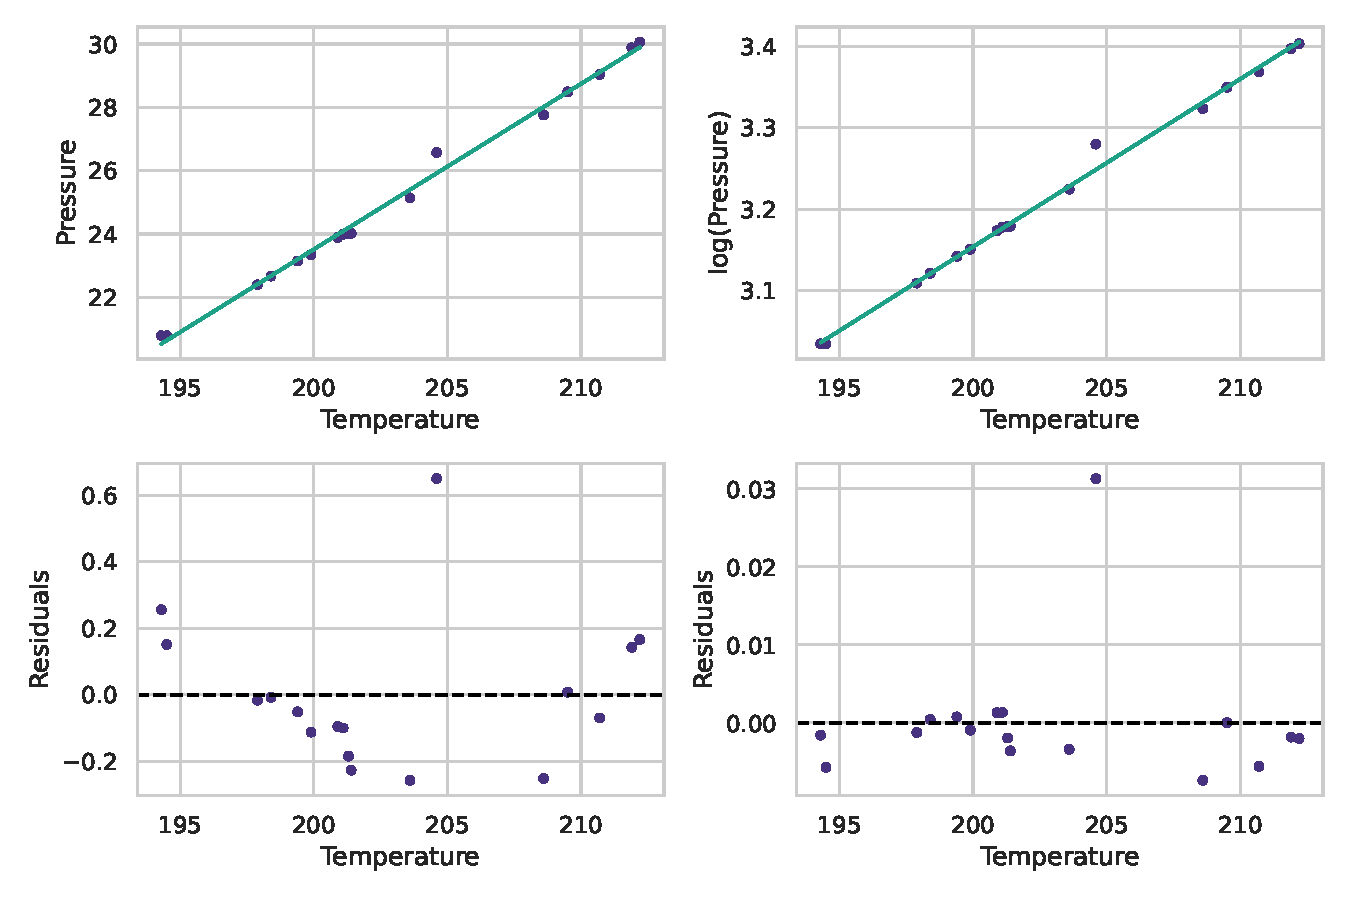
\includegraphics[width=0.9\textwidth]{figures/L06_forbes.pdf}
\caption{Forbes' data. Top: fitted lines for Pressure and for $\log$(Pressure). Bottom: the
corresponding residual plots. Curvature is visible on the left; on the right only case 12 stands out.}
\label{fig:L06-forbes}
\end{figure}

\subsection{A transformation}
The slides then note that \emph{physical theory} says that $\log(\text{Pressure})$ is linearly
related to temperature. We therefore fit
\[
\log(\text{pres}) = a_1 + a_2\,\text{bp}.
\]
With natural logarithms, least squares gives
$\widehat{\log(\text{pres})}=-0.97087+0.020622\,\text{bp}$. The \texttt{alr4} file also contains
\texttt{lpres} $=100\log_{10}(\text{pres})$, which gives $-42.138+0.8955\,\text{bp}$. The two fits
are equivalent up to the constant factor $100/\ln 10$. The residual plot (bottom right) no longer
shows curvature: apart from case~12, the residuals form a horizontal band. Case~12, with residual
$0.0313$ on the log scale, is now clearly an \emph{outlier}. It could be a recording error.

\begin{note}[Supplementary: the physics behind the log]
The Clausius--Clapeyron relation says that the vapour pressure $P$ of a liquid at absolute
temperature $T$ satisfies, approximately, $\log P = c - L/(RT)$. Here $L$ is the latent heat
and $R$ is the gas constant. Water boils when its vapour pressure equals the atmospheric
pressure, so $\log(\text{pres})$ is linear in $1/T$. Over the narrow range
$194$--$212\,^\circ$F (about $363$--$373$\,K), $1/T$ is itself very nearly linear in $T$. This is
why $\log(\text{pres})$ is linear in bp to high accuracy.
\end{note}

\begin{note}[Supplementary: what one outlier does]
Refitting the log model without case~12 gives $\widehat{\log(\text{pres})}=-0.95177+0.020519\,\text{bp}$,
and $R^2$ rises from $0.99496$ to $0.99957$. The slope hardly changes, so the outlier does not
distort the line much. Its main effect is to inflate the residual variance. Whether to delete an
outlier is a scientific decision, not a statistical one. It should be reported either way.
\end{note}

\begin{proposition}[Supplementary: residuals carry no linear trend]\label{prop:L06-noline}
If a least-squares line is fitted to $(x_i,y_i)$, then the least-squares line fitted to the
residual plot $(x_i,\hat e_i)$ is the horizontal line $y=0$.
\end{proposition}
\begin{proof}
By \cref{thm:L05-slr}, the slope for the data $(x_i,\hat e_i)$ is
$\sum_i (x_i-\bar x)(\hat e_i-\bar{\hat e})/S_{xx}$. By \cref{cor:L05-props},
$\bar{\hat e}=0$ and $\sum_i (x_i-\bar x)\hat e_i=0$, so the slope is $0$. The intercept is then
$\bar{\hat e}-0\cdot\bar x=0$.
\end{proof}
So any \emph{linear} tendency is removed by the fit. What remains visible in a residual plot is
non-linear structure (curvature), unequal spread, or unusual points. These are exactly the
features we look for.

\subsection{Computation}
\begin{center}\small
\begin{tabular}{@{}>{\raggedright\arraybackslash}p{7cm}>{\raggedright\arraybackslash}p{8.4cm}@{}}\hline
R & Python\\\hline
\texttt{m <- lm(pres \textasciitilde\ bp, data = forbes)} & \texttt{m = smf.ols("pres \textasciitilde\ bp", data=fb).fit()}\\
\texttt{residuals(m)} & \texttt{m.resid}\\
\texttt{plot(forbes\$bp, residuals(m))} & \texttt{plt.scatter(fb.bp, m.resid)}\\
\texttt{lm(log(pres) \textasciitilde\ bp, data = forbes)} & \texttt{smf.ols("np.log(pres) \textasciitilde\ bp", data=fb).fit()}\\\hline
\end{tabular}
\end{center}
See \nb{week02/L06\_residuals.ipynb}.

\subsection{Summary}
\begin{itemize}
  \item Residual plot: $\hat e_i$ against $x_i$. It should be a structureless band around $0$.
  \item Forbes: $\widehat{\text{pres}}=-81.06+0.523\,\text{bp}$. The residuals are curved, case 12 has the largest positive residual ($0.650$) and case 11 the most negative ($-0.257$).
  \item $\log(\text{pres})$ is linear in bp (physical theory). After transforming, only the outlier (case 12) remains.
  \item The fitted residuals have zero mean and zero correlation with $x$, so only non-linear structure can show up.
\end{itemize}

\subsection{Exercises}
\begin{problem}\label{prob:L06-1}
Show that $\sum_i \hat y_i\hat e_i=0$ for a least-squares line. Deduce that plotting residuals against fitted values also shows no linear trend.
\end{problem}
\begin{problem}\label{prob:L06-2}
Refit Forbes' log model without case $12$ in Python and confirm the coefficients $-0.95177$ and $0.020519$.
\end{problem}
\begin{problem}\label{prob:L06-3}
Show that if $\text{lpres}=100\log_{10}(\text{pres})$, the least-squares coefficients for lpres are exactly $100/\ln 10$ times those for $\ln(\text{pres})$.
\end{problem}
\begin{problem}\label{prob:L06-4}
Describe the residual plot you would expect if the spread of $y$ around the true line grew with $x$.
\end{problem}

\subsection{Further reading}
Weisberg, \emph{ALR}, Chapter~1 (Forbes' data) and Chapter~9 (outliers and diagnostics).
Christensen, Chapter~12 (Model diagnostics).
